\chapter{Uplift Modelling}
\label{ch-uplift}



This chapter is based 
on 
many references,
including Ref.\cite{uplift-2017, fei, wiki-uplift}.

Uphill Modelling (UP)
deals
with  the application of
Rubin's Theory of
Potential Outcomes (PO)
to advertisement and marketing.

PO, which is
discussed in Chapter \ref{ch-po},
 is a subset
of Pearl's Causal Inference.
Besides UP, other  applications of PO theory
that are discussed in this book 
are Regression Discontinuity (Chapter \ref{ch-reg-dis}),
Difference-in-Differences (Chapter \ref{ch-did})
and Synthetic Controls (Chapter \ref{ch-syn-con}).

In UP,
each individual $\s$
is interrogated at two well
anticipated, fairly closely spaced times
$t_0$ and $t_1$ (as opposed to 
Difference-in-Differences  (DID), where
$t_0$ and $t_1$ might
be years apart, and
long after the DID analysis is 
attempted.).
In between those two times,
a treatment which
we will refer to as the
{\bf UP diagnostic test} is applied.
For example,
at times $t_0$ and $t_1$,
each individual
might be asked
how important he/she rates climate 
change on a scale of 1 to 10.
In between times
$t_0$ and $t_1$,
every individual might
be sent a brochure on climate change.
Normally
in PO tests
(for example, in DID),
each individual
$\s$
is either in the 
treated or control
groups, but not both.
But in UP,
the same individual
can be in both the 
treated and control groups.
In UP,
the individuals
are aware  of which
of those groups they are in,
so they are not ``treatment blind".
As explained in 
Chapter \ref{ch-po},
strata matching is only valid
if the subjects
of the test are treatment blind.
Therefore, the only
treatment effect that 
makes sense for UP is SDO,
because it
 does not require strata matching.

\section{UP types}

\begin{figure}[h!]
\centering
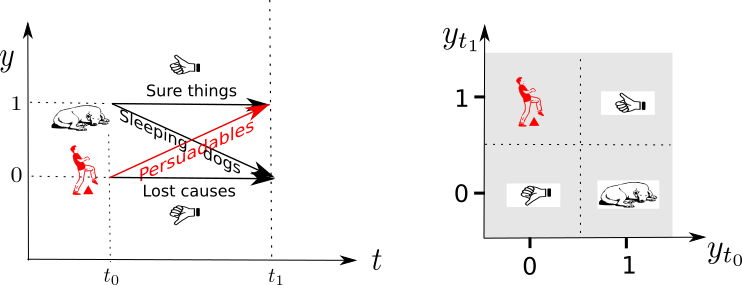
\includegraphics[width=6in]
{uplift/uplift-y-t.png}
\caption{UP diagnostic test
can be used to classify
all individuals of the
population into 4 UP-types.
This figure 
assumes $y^\s\in \bool$.
More generally, $y^\s\in \RR$.
$t$ represents time. $t=t_0$
corresponds to $d^\s=0=untreated$,
and $t=t_1$ corresponds to $d^\s=1=treated$.} 
\label{fig-uplift-y-t}
\end{figure}

Call $\delta^\s_x=
y^\s_{t_1}-y^\s_{t_0}$ the {\bf individual uplift}
for individual $\s$.
As shown
in Fig.\ref{fig-uplift-y-t},
UP classifies individuals
into 4 {\bf UP-types}: Persuadable, SureThings, LostCauses,
and SleepyDogs.
The UP-type
of an individual
depends on the changes 
that are induced on that individual
by an {\bf UP-diagnostic-test}.
\begin{itemize}
\item
For a {\bf Persuadable} individual,
$\delta^\s_x>0$.
\item
For a {\bf SleepyDogs}
individual, $\delta^\s_x< 0$.
\item
For a {\bf SureThings} individual,
 $\delta^\s_x\approx 0$
and $y^\s_{t_0}$ is high.
\item
For a {\bf LostCauses} individual,
$\delta^\s_x\approx 0$
and $y^\s_{t_0}$ is low.
\end{itemize}


Suppose $\s$
belongs to
stratum $A_x$.
What is commonly called 
the {\bf uplift} 
is the {\bf stratum-uplift} $\delta_x=SDO$.
Strata can also be
classified into
the 4 UP-types,
depending on the sign and size  
of their $\delta_x$.
An individual 
may not be typical for
his stratum
and may
have different
{\bf individual and stratum UP-types}.
For example, he may have positive 
individual uplift
and therefore the Persuadable individual UP-type,
but his stratum-uplift
might be negative, so
he belongs to
the SleepyDogs stratum UP-type.

Advertisers are very interested in finding
the Persuadable strata in a population
so as to focus their resources on them.
For example, UP was used very
successfully during the 
Obama presidential campaigns. 
Team Obama conducted UP-diagnostic
tests much like
the climate change one described earlier.
This allowed them to
identify voters who might be sitting on the fence
on whether to vote for Obama or not.
Then they spent
the lion share
of their resources  on those
fence-sitters.


\section{Some Relevant Technical Facts from Chapter \ref{ch-po}}
Some relevant technical facts
about SDO
that were proven in Chapter \ref{ch-po} are

\begin{itemize}
\item
$SDO=0$ is the hypothesis tested 
by a Randomized Clinical Trial (RTC). 

\item
Using $\rvy=\rvy(\rvtd)$
and Fig.\ref{fig-y-diffs-square-probs},
we get

\beqa
SDO &=& \sum_y y\left[
P_{\rvy(1)|\rvtd, \rvx}(y|1, x)
-
P_{\rvy(0)|\rvtd, \rvx}(y|0, x)
\right]
\\
&=&
\sum_y y\left[
P_{\rvy|\rvtd, \rvx}(y|1, x)
-
P_{\rvy|\rvtd, \rvx}(y|0, x)
\right]
\;.
\eeqa
If $\rvy\in \bool$, then

\beq
\underbrace{SDO}_{\displaystyle \delta_x}
=
\underbrace{
P_{\rvy|\rvtd, \rvx}(1|1, x)
}_{\displaystyle \pi^1_x}
-
\underbrace{
P_{\rvy|\rvtd, \rvx}(1|0, x)
}_{\displaystyle \pi^0_x}
\;.
\eeq

\item
Recall that in
Chapter \ref{ch-po}, we used 
$A_{d, x}=\{\s:\td^\s=d,x^\s=x\}$,
$A_x=A_{0,x}\cup A_{1,x}$ and $A=\cup_x A_x$; also
$N_{d,x}=|A_{d,x}|$, $N_x=|A_x|$ and $N=|A|$.
If we substitute
$y^\s\rarrow y^\s(\td^\s)$ and
 $y^{s(\s)}\rarrow y^\s(!\td^\s)$,
where $!0=1$ and $!1=0$, 
into 
the estimator
Eq.(\ref{eq-est-sdo}) for $SDO$,
we get


\beqa
\underbrace{\widehat{SDO}}_{\displaystyle\delta_x}
&=&
\frac{1}{N_{1,x}}
\sum_{\s\in A_x} \td^\s y^\s(\td^\s)
-
\frac{1}{N_{0,x}}
\sum_{\s\in A_x} (1-\td^\s) y^\s(\td^\s)
\\
&=&
\underbrace{\frac{1}{N_{1,x}}
\sum_{\s\in A_{1,x}} y^\s(1)}_
{\displaystyle \pi_x^1}
-
\underbrace{\frac{1}{N_{0,x}}
\sum_{\s\in A_{0,x}}  y^\s(0)}_
{\displaystyle \pi_x^0}
\;.
\label{eq-est-sdo-uplift}
\eeqa

\end{itemize}


\section{UP workflow}

The input
to UP is a PO
dataset $DS= \{ (\s, d^\s, x^\s, y^\s):
 \s=0,1, 1, \ldots, nsam-1\}$.
where $d^\s\in \bool$, $x^\s \in S_\rvx$,
$y^\s\in \RR$.
 Individuals
with $d^\s=0$ and $d^\s=1$
are considered 
different individuals.
We will assume 
$S_\rvx$ is a finite set.
In general,
$x=(x_0, x_1,\dots, x_{n-1})$ is an $n$ dimensional 
vector of features $x_i$.
If any of the $x_i$
is a priori continuous, we will
assume it has  been binned into
a finite number of bins.

\begin{figure}[h!]
\centering
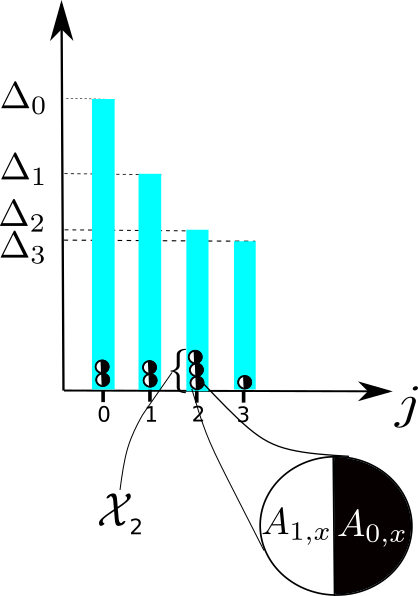
\includegraphics[width=2in]
{uplift/uplift-bins.png}
\caption{
Pictorial
representation
of the sequence
$\{(\calx_j, \Delta_j)\}_{j=0,1, \ldots, nj-1}$.
}
\label{fig-uplift-bins}
\end{figure}


Starting with $DS$,
UP performs the following steps.
Fig.\ref{fig-uplift-bins}
is a pictorial representation
of the quantities
that are calculated
during these steps.

\begin{enumerate}
\item Find $A_x$ 
for each observed $x\in S_\rvx$.
Set $A_x=\emptyset$ for unobserved $x\in S_\rvx$.
 
\item Calculate $\delta_x$
for each $x\in S_\rvx$.
Set $\delta_x=0$ if $A_x=\emptyset$.

\item Calculate
the set $\{\Delta_j\}_{j=0, 1, \ldots, nj-1}$
of distinct uplifts $\delta_x$.
The labels 
$j$ should be assigned
so that the sequence of
$\Delta_j$
is monotonically non-increasing; i.e.,
$\Delta_0 \geq \Delta_{1}\geq\cdots \geq \Delta_{nj-1}$.
 $\Delta_j = \Pi_j^1-\Pi_j^0$
since $\delta_x=\pi^1_x - \pi^0_x$.
Now calculate
$\calx_j =\{ x: \delta_x =\Delta_j\}$ for each $j$.
By the end of this step,
we will have calculated 
$\{(\calx_j, \Delta_j)\}_{j=0,1, \ldots, nj-1}$.
We will refer to the $\calx_j$
as {\bf strata-bins}.
\item
For each $j$,
calculate $\Sigma_{d,j}=\cup_{x\in \calx_j}A_{d,x}$
for $d\in\bool$
and $\Sigma_{j}=\Sigma_{0,j}
\cup \Sigma_{1,j}$.
\end{enumerate}


\begin{figure}[h!]
\centering
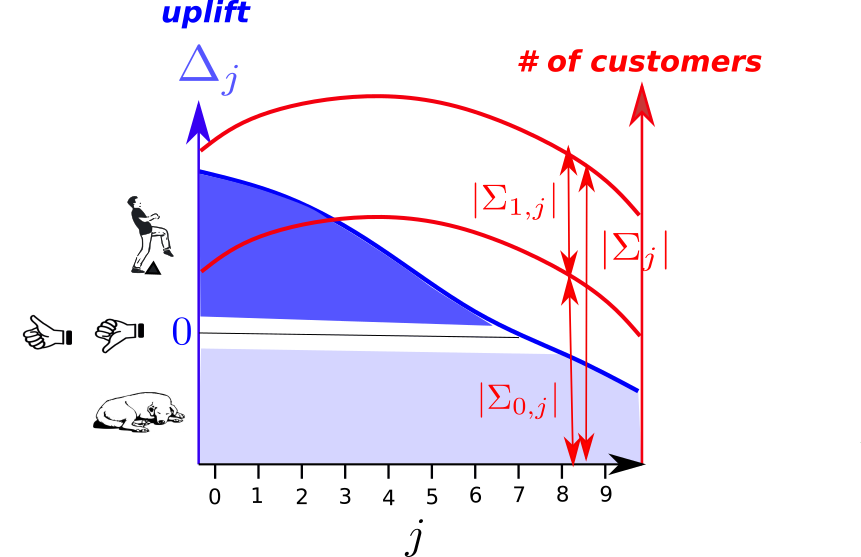
\includegraphics[width=4.5in]
{uplift/qini-fake.png}

\caption{
Plot
of UP results.
Sane alternative to Qini curves.
} 
\label{fig-qini-fake}
\end{figure}
Fig.\ref{fig-qini-fake}
is a  way of
plotting
the results 
of UP in an
intuitive
way
that even a
business type can grok.
UP software
often plots something
called a Qini
curve, 
but I find Qini
curves opaque, confusingly defined 
in the literature, unnecessary
and 
not very well motivated. So I don't
use or recommend them.




\section{Finding 
$\{({\cal X}_j, \Delta_j)\}_{0,1, \ldots, nj-1}$ with decision trees}
